\part{Seminar 5 - Comparison of hybrid analytical modelling and reluctance
network modelling for pre-design purposes}

\makebox[.25\textwidth]{Antoine Lemaire}\makebox[.25\textwidth]{Lucas Morettin}\makebox[.25\textwidth]{Louis Peeters}\makebox[.25\textwidth]{Lucas Pousseur}

\section*{Abstract}

Le but du document est de comparer la modelisation hybride analytique avec réseau de reluctance vs réseau de reluctance generée sur base du maillage (Mesh-based generated reluctance network) pour une structure linéaire à aimants permanents. Les critères de comparaison sont : \begin{itemize}
    \item Le temps de calcul
    \item La qualité des résultats
\end{itemize} 
Ce deux méthodes seront comparées à la méthode des éléments finis que l'on considère comme base correcte de résultats. Pourquoi? Pour montrer que l'on peut coupler les résultats de la modelisation analytique et de la modelisation par réseau de reluctance.
\section{Introduction}
En général, le pre-design des structures electriques sont faites par éléments finis car ils apportent des résultats précis. Mais ils requierent beaucoup de calculs et donc beaucoup de temps. Il y a deux alternatives utilisées pour éviter ces inconvénients : 
\begin{itemize}
    \item Méthode des réseaux de reluctance (méthode semi-numérique) (Séminaire 1)
    \item Méthode analytique (Séminaire 2)
\end{itemize}
Ici, on va mixer les 2 pour la méthode hybride.
\section{Moteur linéaire}
\textit{(Cette partie n'est presque pas détaillée dans le doc, je sais pas si il pose les questions sur la matière de la présentation ou juste sur la matière du document mais je met tout ce que j'ai dis à la présentation au cas où)}\\
C'est le même principe que le moteur electrique sauf qu'on met à plat le stator et le rotor. La configuration des bobines est la suivante :

\begin{figure}[H]
    \centering
    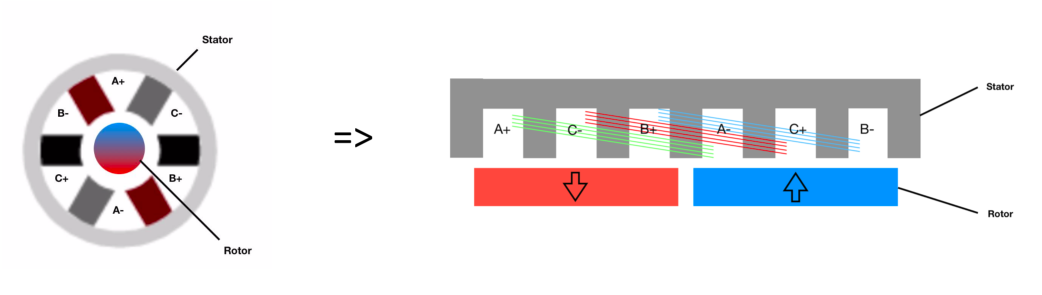
\includegraphics[scale=.4]{Bobinage.png}
    \caption{Configuration bobinages (Gauche: moteur electrique tournant, droite: moteur electrique linéaire)}

\end{figure}

Le stator est lui constitué d'aimants permanents avec la paire de pôle représentée ici en rouge et bleu.

\subsection*{Forces}
Le but de cette configuration est de produire une force linéaire (à la place d'un couple de rotation pour les machines tournantes). 
Pour avoir un mouvement linéaire, on va injecter du courant triphasé équilibré dans les bobines avec un certaine fréquence $f$. Cela va créer un champ magnétique "glissant" sur l'entrefer qui va interagir avec le champs magnétique des aimants permanents. Cette interaction va entrainer une force de poussée linéaire qui va faire bouger le rotor dans cette direction.

Mais ce n'est pas la seule force qui agit dans ce type de structure. Il y a aussi la force d'attraction (Cogging force) qui elle n'est pas due au courant due à l'interaction entre le stator et les aimants permanents sans courant. Elle est représentée sur le schéma suivant :

\begin{figure}[H]
    \centering
    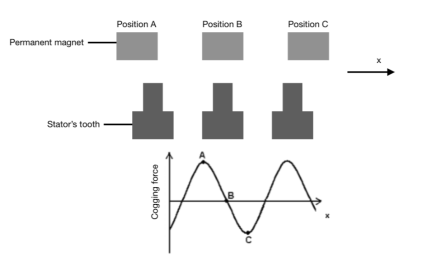
\includegraphics[scale=.6]{Cogging.png}
    \caption{Représentation de la force d'attraction (sans courant)}

\end{figure}

On a donc en résumé deux forces majeures, misent en valeur dans la formule suivante pour les moteurs tournants mais correspondantes à des forces linéaires dans notre configuration(force reluctante négligeable) : 
\begin{figure}[H]
    \centering
    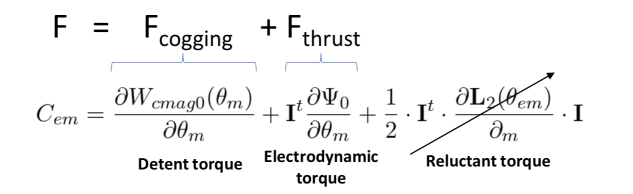
\includegraphics[scale=.6]{Forces.png}
    \caption{Forces de la structure}
\end{figure}
Elles ont pour définition : 
\begin{itemize}
    \item Force de poussée : Due à l'interaction entre le courant des bobines du stator et le flux induit par les aimants permanents du rotor à travers ces bobines.
    \item Force d'attraction : Due à l'interaction entre le stator et l'aimant permanent sans courant.
\end{itemize}
\subsection*{Vitesse}
On calcule la vitesse du rotor avec la formule suivante : 
\begin{center}
    $V_s = 2\tau_p \cdot f$
\end{center}
avec : 
\begin{itemize}
    \item $V_s$ la vitesse synchrone linéaire du champs magnétique [m/s]
    \item $f$ la fréquence du courant [Hz]
    \item $\tau_p$ le pas polaire de l'aimant permanent (pole pitch) [m] représenté sur la figure \ref{polepitch}
\end{itemize}
\begin{figure}[H]
    \centering
    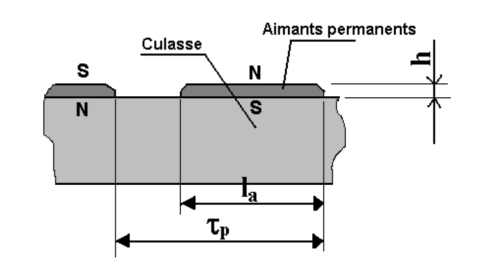
\includegraphics[scale=.6]{Polepitch.png}
    \caption{Représentation du pas polaire $\tau_p$}
    \label{polepitch}

\end{figure}
\subsection*{Hypothèses pour la modelisation}
\begin{itemize}
    \item Le stator et le rotor sont des structures périodiques donc on a pas d'effets de bords
    \item Le champs magnétique est considéré comme \begin{itemize}
        \item Normal entre le stator et les aimants permanent
        \item Tangentiel à l'interface air-stator
    \end{itemize}
\end{itemize}

\begin{figure}[H]
    \centering
    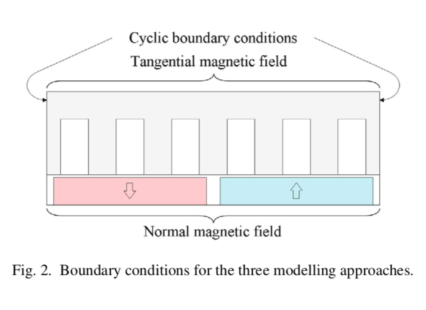
\includegraphics[scale=.5]{ConditionsLimites.png}
\end{figure}

\subsection*{Exemples d'application}
\begin{itemize}
\item Train à lévitation magnétique
\item Actionneurs linéaires utilisés en automatique et robotique
\end{itemize}
\section{Modélisation par réseau de réluctance}
\subsection{Principe}
Lors du pre-design d'une machine, le modèle à réseau de réluctance (RN) peut être utilisé pour modéliser sa structure. \textbf{Ce modèle RN repose sur un maillage de la structure étudiée à base de circuits magnétiques réluctants, couplé à l'algorithme présenté en figure X afin de calculer le flux traversant toute la structure} ; et ainsi déterminer les propriétés magnétiques adéquates des matériaux qui satisferont le parfait fonctionnement de la future machine.

\begin{center}
 \textit{"This method consists in the meshing of the studied domain with regular volumes, each of
them modelled by a local reluctance network"} 
\end{center}

Dans ce séminaire, nous nous concentrons sur la modélisation d'une machine linéaire à aimants permanents et traiterons donc uniquement d'éléments rectangulaires utilisé pour le maillage. Néanmoins le principe reste identique pour des éléments de géométries différentes.

\subsection{Développement d'un élément du maillage (2D)}

Le développement du maillage d’un réseau de réluctance revient à une décomposition de la structure en
un ensemble de tubes de flux.

\subsubsection{Décomposition en éléments unidirectionnels}
De prime à bord, chaque élément du maillage est modélisé par un tube de flux auquel est associé un circuit magnétique unidirectionnel (celui-ci se compose d'une réluctance ainsi que d'éventuelles sources). Cette modélisation par réluctance au niveau du tube de flux introduit une fixation des trajectoires de flux, ce qui introduit une réduction de la flexibilité du modèle.

Cet inconvénient apparait dans le cas de la modélisation des machines électriques et surtout
dans les parties où les lignes de flux varient selon l’état magnétique de la machine, et par
conséquent les tubes de flux changent. Ce qui est le cas pour la partie inférieure de la dent où
les lignes de flux changent en fonction de la position du rotor et du niveau de saturation

\subsubsection{Décomposition en éléments multidirectionnels}
Pour résoudre ce problème, un maillage même du tube de flux est utilisé. Cette méthode consiste à
décomposer chaque élement en quatre branches (au lieu d'une), nous introduisons ainsi une flexibilité du
passage de flux : le flux peut traverser un élément dans différentes directions et non plus
une seule. Les branches de chaque bloc sont reliées entre elles par un nœud central $i$ et aux branches des blocs voisins par quatre nœuds latéraux $j=1,2,3,4$. Chaque branche est constituée d'une réluctance éventuellement couplée à des
sources de FMM et de flux, ceci dépendant du milieu à modéliser.

\begin{figure}[H]
    \centering
    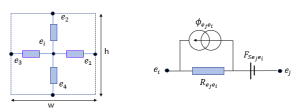
\includegraphics[scale=.8]{element.png}
    \caption{Schéma géneral d'un élément du maillage (gauche) et d'une de ses branche (droite)}
\end{figure}

\subsection{Géométrie de l'élément}
La géométrie des éléments choisis pour le maillage dépend directement de la structure à modéliser : 

\begin{itemize}
    \item Structure 2D (élément 2D) ou 3D (élément 3D)
    \item Structure à géométrie rectangulaire (élément rectangulaire) ou complexe (élément triangulaire, hexagonal, ...)
    \item Comportement du flux dans le milieu à modéliser (élément uni(multi)-directionnel)
\end{itemize}

\subsection{Modélisation de la structure}
Dans le cadre de ce séminaire, la structure étudiée est une machine linéaire à aimants permanents ; la méthode RN implique de modéliser sa structure par un maillage composé d'éléments rectangulaires. Néanmoins les propriétés de ces éléments peuvent différer en fonction de la partie de la structure qu'ils modélisent.

C'est pourquoi dans cette section nous développons physiquement et mathématiquement les différents types d'élements qui composerons le maillage et donc modéliserons distinctement le stator, la partie mobile et l'entrefer de la machine.

\subsubsection{Modélisation de l'entrefer}
La modélisation de l’entrefer présente une importance cruciale, puisque c’est le lieu de
conversion de l’énergie (électrique $\iff$ mécanique).

Lors de sa modélisation, deux types d’éléments peuvent être utilisés : des
éléments unidirectionnels ou des
éléments multidirectionnels. Le choix du type d’éléments dépend des grandeurs globales que l’on désire
estimer (flux ou couples (ou forces)) et de la précision souhaitée.\\
En ce qui nous concerne pour le calcul du
flux d’entrefer, l’utilisation d’éléments unidirectionnels est souvent suffisante,
particulièrement si l’entrefer est faible De plus, l’utilisation d’éléments unidirectionnels dans
l’entrefer implique un nombre de nœuds plus faible, en comparaison de l’utilisation
d’éléments multidirectionnels, et par conséquent, un temps de calcul plus réduit.\\
D'un autre côté, l'entrefer étant la portion de la structure la plus importante à modéliser, l'utilisation d'une haute densité d'éléments bidirectionnels favoriserait grandement la précision, quitte à allonger le temps de calcul. Le choix du type d'élément résulte donc d'un compromis.

\subsubsection*{Prise en compte du mouvement}

La figure X  montre comment la valeur de la réluctance
d’entrefer, reliant un élément statique et un élément appartenant à la partie mobile, est estimée
en fonction de la position relative de la partie mobile par rapport à la partie fixe. Pour des
raisons de clarté, seulement un élément du stator $e_1$ et un élément de la partie mobile $e_2$ y sont
représentés.

La valeur de la réluctance de l’élément unidirectionnel entre les deux éléments $e_1$ et $e_2$ est
estimée par la formule suivante :

\begin{equation}
    R_{e_2e_1}^{ag} = \frac{1}{\mu_0}\frac{h}{l_a\Delta v}
\end{equation}

où, $h$ est l’épaisseur de l’entrefer, $L_a$ est la longueur axiale des éléments (les deux éléments
possèdent la même longueur axiale), et l’expression de $\Delta v$ est donnée par :

\begin{equation}
    \Delta v = \alpha(v_{e_12}-v_{e_21})+\beta(v_{e_22}-v_{e_11}) -\alpha\beta(v_{e_12}-v_{e_1})
\end{equation}

avec

\[
\alpha = \left\{
\begin{array}{l c l}
1, \text{ si } v_{e_11}\leq v_{e_21}\leq v_{e_12}\\
0, \text{ sinon}\numberthis
\end{array}
\right.
\]
\[
\beta = \left\{
\begin{array}{l c l}
1, \text{ si } v_{e_11}\leq v_{e_22}\leq v_{e_12}\\
0, \text{ sinon}\numberthis
\end{array}
\right.
\]

\subsubsection*{Modèle d'un élément $i$ d'entrefer}
Nous pouvons maintenant modéliser un élement $i$ unidirectionnel/multidirectionnel composant le maillage de l'entrefer et y associer les équations magnétiques correspondant. Pour $h$ l'épaisseur et $L_a$ est la longueur axiale de l'élément $i$, 

\begin{itemize}
    \item \textbf{Element unidirectionnel}
        \begin{equation}
            U_{e_j}-U_{e_i}=R_{e_je_i}^{ag}\Phi_{e_je_i} \qquad \text{ pour } j=1
        \end{equation}
        avec
        \begin{equation}
            R_{e_je_i}^{ag} = \frac{1}{\mu_0}\frac{h}{l_a\Delta v}
        \end{equation}
    
    \item \textbf{Elément multidirectionnel}
        \begin{equation}
            U_{e_j}-U_{e_i}=R_{e_je_i}^{ag}\Phi_{e_je_i} \qquad \text{ pour } j=1,2,3,4
        \end{equation}
        avec
        \[
        \left\{
        \begin{array}{l c l}
        R_{e_1e_i}^{ag}=R_{e_3e_i}^{ag} = \frac{1}{\mu_0}\frac{\Delta v/2}{l_ah}\\
        R_{e_2e_i}^{ag}=R_{e_4e_i}^{ag} = \frac{1}{\mu_0}\frac{h/2}{l_a\Delta v}\numberthis
        \end{array}
        \right.
        \]
        
\end{itemize}


\subsubsection{Modélisation de la partie mobile}
Les aimants permanents sont modélisés par des sources de flux en parallèle avec une réluctance constante. La valeur de la source de flux est égale à l’induction rémanente
multipliée par la surface de l’aimant traversée par le flux. Ce modèle est simple à implémenter dans un réseau de réluctances pour n’importe quel positionnement des aimants au niveau de la machine.

\subsubsection*{Modèle d'un élément $i$ de la partie mobile}
Ainsi, chaque aimant permanent appartenant à la machine linéaire étudiée peut être maillé à l'aide de l'élément suivant  : 

\[
\left\{
\begin{array}{l c l}
U_{e_j}-U_{e_i}=R_{e_je_i}(\Phi_{e_je_i}-\Phi_{Se_je_i}) \qquad \text{ pour } j=2,4 \\
U_{e_j}-U_{e_i}=R_{e_je_i}\Phi_{e_je_i} \qquad \qquad\qquad  \text{ pour } j=1,3 \numberthis
\end{array}
\right.
\]
avec
\[
\left\{
\begin{array}{l c l}
R_{e_2e_i}=R_{e_4e_i}=\frac{1}{\mu_0\mu_r}\frac{h/2}{wl_a}\\
\Phi_{Se_2e_i}=\Phi_{Se_4e_i}=B_Rwl_a\\
R_{e_1e_i}=R_{e_3e_i}\frac{1}{\mu_0\mu_r}\frac{w/2}{hl_a} \numberthis
\end{array}
\right.
\]

\subsubsection{Modélisation du stator}
La 2ème source présente dans les machines électriques est le courant circulant au niveau des
bobinages. Ceux-ci sont modélisés par des sources de FMM
selon la direction normale au plan de bobinage, la valeur maximale de la FMM est $FFM_{max}=NI=NJ_SA$.

\begin{figure}[H]
    \centering
    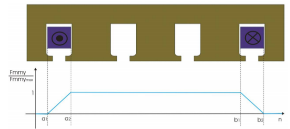
\includegraphics[scale=.7]{stator.png}
    \caption{Présentation de la distribution des bobinages et des FMM normalisées}
    \label{stator}
\end{figure}

Nous prenons l’exemple d’un bobinage de notre machine linéaire en \textsc{Figure \ref{stator}}. Pour la partie statorique
blocs située entre les deux encoches de bobinage la FMM est égale à sa valeur maximale.

\begin{figure}[H]
   \begin{minipage}[c]{.45\linewidth}
        \centering
              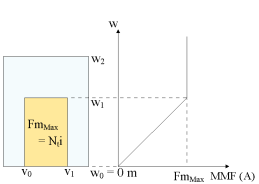
\includegraphics[scale=1]{stator1.png}
              \caption{Variation de la FMM}
            \label{stator2}
   \end{minipage} \hfill
   \begin{minipage}[c]{.45\linewidth}
      \centering
      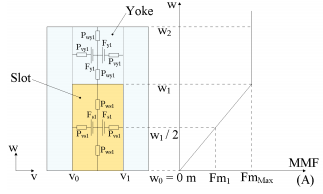
\includegraphics[scale=0.7]{stator2.png}
      \caption{Maillage initial d’une encoche et de la culasse}
    \label{stator1}
   \end{minipage}
\end{figure}

La \textsc{Figure \ref{stator1}} montre la variation de la FMM en fonction de la coordonnée $w$ (axe $y$) pour une bobine. La \textsc{Figure \ref{stator2}} montre le maillage initial avec
les éléments contenant les branches actives contenant les sources de FMM représentant les
conducteurs. Toutes les sources de FMM utilisées pour modéliser les enroulements
sont localisées sur les branches horizontales, parallèles à l’entrefer :
\begin{align*}
    F_{s1} &= \frac{Fm_1}{2} = \frac{Fm_{Max}}{4}= \frac{NI}{4}\\ \numberthis
    F_{y1} &= \frac{Fm_{Max}}{2} = \frac{NI}{2} 
\end{align*}



La \textsc{Figure \ref{stator3}} montre un exemple d’affinage pour avoir une variation plus réaliste de la FMM en fonction de la coordonnée $w$, et un meilleur maillage de l’entrefer.
Les valeurs des sources de FMM, pour les différents éléments $e_{s1}$, $e_{s2}$, $e_{s3}$ et $e_{y1}$, dépendent de la géométrie (forme et dimensions géométriques) de chaque élément et de la valeur du
courant.

\begin{figure}[H]
    \centering
    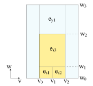
\includegraphics[scale = 1]{stator3.png}
    \caption{Affinage du maillage}
    \label{stator3}
\end{figure}

 Les expressions des sources de FMM pour ces éléments sont données par : 
 
 \[
\left\{
\begin{array}{l c l}
Fm_{e_s1}=\frac{(w_1-w_0)(v_1-v_0)}{4(w_2-w_0)(v_2-v_0)}Fm_{Max}\\
Fm_{e_s2}=\frac{(w_1-w_0)(v_2-v_1)}{4(w_2-w_0)(v_2-v_0)}Fm_{Max}\\
Fm_{e_s3}=\frac{(w_2+w_1-w_0)}{4(w_2-w_0)}Fm_{Max}\\
Fm_{e_y1} = \frac{Fm_{Max}}{2}\numberthis
\end{array}
\right.
\]


Maintenant que nous pouvons déterminer la FMM produite par un bobinage en tout point du stator, nous pouvons y associer les équations servant au calcul du flux dans cette région de la machine.

\subsubsection*{Modèle d'un élément $i$ du bobinage}
\[
\left\{
\begin{array}{l c l}
U_{e_j}-U_{e_i}=R_{e_je_i}\Phi_{e_je_i}-F_{Se_je_i} \qquad \text{ pour } j=1,3 \\
U_{e_j}-U_{e_i}=R_{e_je_i}\Phi_{e_je_i} \qquad \qquad\qquad  \text{ pour } j=2,4 \numberthis
\end{array}
\right.
\]
avec
\[
\left\{
\begin{array}{l c l}
R_{e_2e_i}=R_{e_4e_i}=\frac{1}{\mu_0\mu_r}\frac{h/2}{wl_a}\\
F_{Se_1e_i}=F_{Se_3e_i}=NJ_swh/4\\
R_{e_1e_i}=R_{e_3e_i}\frac{1}{\mu_0\mu_r}\frac{w/2}{hl_a} \numberthis
\end{array}
\right.
\]

\subsubsection*{Modèle d'un élément $i$ de culasse}
\[
\left\{
\begin{array}{l c l}
U_{e_j}-U_{e_i}=R_{e_je_i}\Phi_{e_je_i}-F_{Se_je_i} \qquad \text{ pour } j=1,3 \\
U_{e_j}-U_{e_i}=R_{e_je_i}\Phi_{e_je_i} \qquad \qquad\qquad  \text{ pour } j=2,4 \numberthis
\end{array}
\right.
\]
avec
\[
\left\{
\begin{array}{l c l}
R_{e_2e_i}=R_{e_4e_i}=\frac{1}{\mu_0\mu_r}\frac{h/2}{wl_a}\\
F_{Se_1e_i}=F_{Se_3e_i}=NJ_swh/2\\
R_{e_1e_i}=R_{e_3e_i}\frac{1}{\mu_0\mu_r}\frac{w/2}{hl_a} \numberthis
\end{array}
\right.
\]
\subsection{Formulation du système d'équation}
L’approche nodale est adoptée pour la formulation du système d’équations lié au modèle RN. Les
inconnues de ce système sont les valeurs du potentiel scalaire magnétique aux
nœuds. Ce système d’équations est exprimé sous forme matricielle, comme suit :

\begin{equation}
    [M]\cdot[U]=[\phi]
\end{equation}

où, $[M]$ $[n \times n]$ est la matrice associée aux réluctances, $[U$] $[n \times 1]$ est le vecteur des
inconnues (potentiel scalaire magnétiques aux nœuds), et $[\phi]$ $[n \times 1]$ est le vecteur des
sources du système.

Pour chaque position relative de la partie mobile par rapport au stator, on génère un nouveau système
d’équations. Il faut noter que seul l’entrefer est remaillé à chaque pas de
mouvement.

\begin{figure}[H]
    \centering
    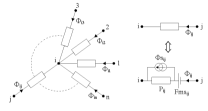
\includegraphics[scale=.9]{form.png}
    \caption{Réseau de réluctance pour le $i$ème noeud}
    \label{kirc}
\end{figure}

La \textsc{Figure \ref{kirc}} illustre comment le système est déterminé à partir des lois de Kirchoff. En effet nous associons, à chaque élément $i$ du maillage, une équation nodale obtenue par l'application des lois de Kirchoff, prenant en compte l'influence (les échanges de flux) des éléments lui étant adjacents. Ainsi, pour tout élément $i$ du maillage : 


\[
\left\{
\begin{array}{l c l}
\sum \limits_{\underset{j \neq i}{j=1}}^n \Phi_{ij} = 0 \text{Wb}\\
U_i-U_j = F_{S_{ij}}-(\Phi_{ij}-\Phi_{s_{ij}})M_{ij}\numberthis
\end{array}
\right.
\]
\newpage
En subtituant, nous trouvons une équation nodale unique caractérisant le noeud $i$ : 

\begin{equation}
    \left(\sum \limits_{\underset{j \neq i}{j=1}}^n M_{ij}\right)U_i+\sum \limits_{\underset{j \neq i}{j=1}}^n \left(-U_jM_{ij}\right)=\sum \limits_{\underset{j \neq i}{j=1}}^n \left(\Phi_{S_{ij}}+F_{S_{ij}}M_{ij}\right)
\end{equation}

Où les éléments des matrices $[M]$ (qui est en fait la matrice des perméances\footnote{Voir équation (2) du document de référence sur Moodle}) et $[\Phi]$ peuvent directement être directement déterminés en utilisant les équations (6), (8), (10), (14) et (16). Pour les nœuds $j$ qui ne sont pas directement connectés au noeud $i$, les
valeurs de $M_{ij}$, $F_{S_{ij}}$ et $\Phi_{S_{ij}}$ sont nulles.

\subsubsection{Conditions frontières}
Il ne faut pas oublier de prendre en compte les conditions frontières dans la résolution du système d'équation. Ainsi,

\begin{itemize}
    \item Le \textit{champ magnétique tangentiel à l'interface stator-air} est satisfait en modélisant y modélisant les éléments par des réluctances horizontales.
    \item Le \textit{champ magnétique normal à l'interface aimant permanent-partie mobile} est satisfait par le potentiel scalaire magnétique nul fixé à cette interface précédemment.
\end{itemize}

\begin{figure}[H]
    \centering
    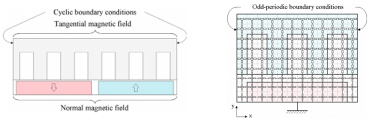
\includegraphics[scale=.8]{front.png}
    \caption{Conditions frontières}
\end{figure}

\subsubsection{Résolution du système}
Le système (17) peut alors être résolu afin de déterminer les valeurs de potentiel magnétique scalaire $U$ en tout noeud du maillage. Finalement, c'est en remplaçant ces valeurs $U$ dans les équations (5), (7), (9), (13) et (15) que le flux traversant chaque branche d'élément peut-être déterminé.

\newpage
\subsection{Algorithme de résolution et prise en compte de la saturation magnétique}
\subsubsection{Saturation magnétique}
Afin de tenir compte de la saturation magnétique, le système d’équations est résolu de
manière itérative, en ajustant à chaque itération les valeurs des éléments de la matrice des
réluctance $[M]$. Le critère de convergence est défini par :
\begin{equation}
    \frac{[\mu_e^{k+1}-\mu_e^k|}{\mu_e^k}<1\%
\end{equation}

où, $\mu_e^k$ et $\mu_e^{k+1}$ correspondent aux valeurs de la perméabilité relative dans l'élément de réluctance $e$ aux itérations $k^{th}$ et $k^{th}+1$ respectivement.

Le calcul de la perméabilité relative d’un élément est effectué par l’intermédiaire du calcul de
l’énergie magnétique de l’élément en question. Ce calcul n'est pas détaillé lors de ce séminaire.
Le principal intérêt d'ajuster les matrices de réluctance pour matcher le critère de convergence est de déterminer les caractéristiques des matériaux qui seraient à même d'être utiliser dans la conception de la machine. 

\subsubsection{Algorithme}
La figure \textsc{Figure \ref{algo}} donne l’algorithme de l’approche de modélisation adoptée, en considérant la
saturation magnétique et le mouvement de la partie mobile. 

\begin{figure}[H]
    \centering
    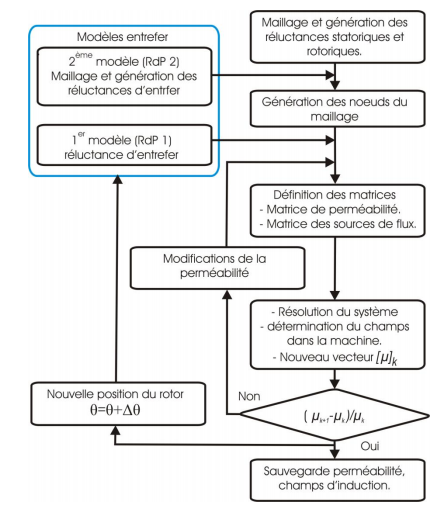
\includegraphics[scale=.8]{algo.png}
    \caption{Algorithme du modèle à réseau de réluctance}
    \label{algo}
\end{figure}

\subsubsection*{Remarque}
Le pas de mouvement minimum est choisi de façon à correspondre à la distance entre deux noeuds adjacents du maillage.


\section{Hybrid analytical modelling}
La méthode hybride consiste a coupler les deux méthodes (réseaux de reluctance et méthode analytique(basé sur la solution des équations de maxwell, on modélise le stator en réseau de reluctance tandis que l'entrefer et les aimants permanents sont modélisé par la méthode analytique. Il faut par la suite coupler les deux méthodes au condition limite et résoudre un système pour avoir la modélisation complète. Cette méthode a l'avantage d'éviter de devoir modéliser l'entrefer avec un réseaux de reluctance(compliqué), par contre cela a un cout en effet il faut faire des hypothèses radicale notamment considérer la partie inféreur aux aimants comme ayant une perméabilitité magnétique infinie et donc ne pas tenir compte de la saturation.
\subsection{méthode analytique}
Comme expliqué ci-dessus, on applique la méthode analytique sur l'entrefer et les aimants permanents.
\begin{figure}[H]
    \centering
    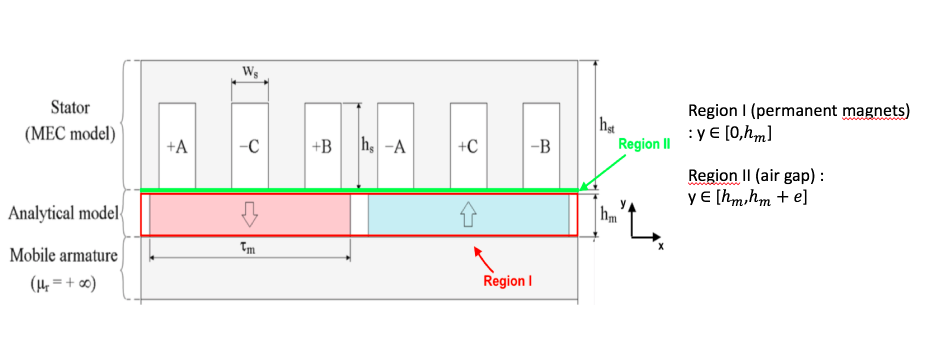
\includegraphics[scale=0.4]{schemahybrid.png}
    \caption{schema du moteur}
    \label{hyb}
\end{figure}


\subsection{Potentiel scalaire par région}
Les vecteurs $B$ et $H$ sont liés par

\[
\left\{
\begin{array}{r c l}
B &=& \mu_0(H+M), \qquad \text{pour la région I}\\
B &=& \mu_0H, \qquad \text{pour la région II}
\end{array}\numberthis
\right.
\]
On a l'equation ci dessous [\ref{amperLaw}](ampere law) car aucun courant n'est présent dans le rotor, et par définition un champ vectoriel irrotationnel peut etre identifié comme étant égal à la divergence d'un potentiel scalaire.
\begin{equation}
  \nabla xH=0
  \label{amperLaw}
\end{equation}
Le vecteur champ magnétique $H$ est donné par la définition du potentiel scalaire : 

\begin{equation}
    H = -\nabla U = -\frac{\partial U}{\partial x}\overline{e}_x -\frac{\partial U}{\partial y}\overline{e}_y
\end{equation}

Pour la structure étudiée, les aimants permanents sont magnétisés selon la direction $y$ ($M_x = 0)$, le potentiel magnétique scalaire $U$, dans les régions I et II, est alors régit par l'équation suivante : 

\begin{equation}
    \Delta U = \frac{\partial^2U}{\partial x^2}+\frac{\partial^2U}{\partial y^2} = 0
\end{equation}

Le potentiel scalaire $U$ dans la région des aimants permanents (région I, $y\in[0, h_m]$) et celle de l'entrefer mécanique (région II, $y\in[h_m, h_m+e]$) est régie par l'équation suivante

\[
\left\{
\begin{array}{r c l}
\Delta U &=& \frac{\partial^2U}{\partial x^2}+\frac{\partial^2U}{\partial y^2} = \nabla\cdot M, \qquad \text{pour la région I}\\
\Delta U &=& \frac{\partial^2U}{\partial x^2}+\frac{\partial^2U}{\partial y^2} = 0, \qquad \text{pour la région II}\\ \numberthis
\end{array}
\right.
\] 


où $M$ est le vecteur de magnétisation, donc les composantes peuvent être exprimées, dans le repère cartésien, en séries de Fourier comme suit

\[
\left\{
\begin{array}{r c l}
M_x &=& \sum_{n=1}^\infty(M_{x1n}sin(n\pi x/\tau_p)+M_{x2n}cos(n\pi x/\tau_p))\\
M_y &=& \sum_{n=1}^\infty(M_{y1n}sin(n\pi x/\tau_p)+M_{y2n}cos(n\pi x/\tau_p))\numberthis
\end{array}
\right.
\]



En effet $M_x$ et $M_y$, les composantes de $M$, sont uniquement fonction de $x$. Dès lors :

\begin{equation}
    \nabla\cdot M = \frac{\partial M_x}{\partial x}+\frac{\partial M_y}{\partial y} = \frac{\partial M_y}{\partial y} = 0
\end{equation}

et

\[
\left\{
\begin{array}{r c l}
\Delta U &=& \frac{\partial^2U}{\partial x^2}+\frac{\partial^2U}{\partial y^2} = \nabla\cdot M=0, \qquad \text{pour la région I}\\ \numberthis
\Delta U &=& \frac{\partial^2U}{\partial x^2}+\frac{\partial^2U}{\partial y^2} = 0, \qquad \text{pour la région II}\\ 
\end{array}
\right.
\]

La solution générale de cette équation de Laplace peut être exprimée pour un région i par 

\begin{align*}
    U^{(i)}(x,y) &= a_0^{(i)}+a_1^{(i)}x+a_2^{(i)}y+a_3^{(i)}xy\\
    &+\sum_{n=1}^\infty \left(a_{4n}^{(i)}sinh(\frac{n\pi y}{\tau_p})+a_{5n}^{(i)}cosh(\frac{n\pi y}{\tau_p})\right)sin(\frac{n\pi x}{\tau_p})\\
    &+ \left(a_{6n}^{(i)}sinh(\frac{n\pi y}{\tau_p})+a_{7n}^{(i)}cosh(\frac{n\pi y}{\tau_p})\right)cos(\frac{n\pi x}{\tau_p})\numberthis
\end{align*}


\begin{center}
    Voir résolution équation de Laplace dans un rectangle (Math 3)\\ Superposition de l'ensemble des n solutions de chaque cas\footnote{\url{http://web.mit.edu/course/6/6.013_book/OldFiles/www/chapter5/5.4.html}}\\
\end{center}
En considérant les symétries géométriques et la périodicité électromagnétique de la structure étudiée\footnote{\url{https://quickfield.com/help/QuickField.chm/html/Data/PeriodicBoundaryConditions.htm}}, il est facile de montrer que $a_1^{(i)}=a_2^{(i)}=a_3^{(i)}=0$ pour les deux régions. $a_0^{(i)}$ est une constante arbitraire qui peut être choisie nulle. On a donc pour chaque région $4N_h$ inconnues ou $N_h$ est le nombre d'harmonique de la série de fourier. ($a_{4n},a_{5n},a_{6n},a_{7n}$).

%\begin{figure}[H]
%    \centering
%    \includegraphics[scale=1.2]{mh2.png}
%    \caption{Conditions limites appliquées à la structure.}
%\end{figure}

\subsubsection{Région des aimants permanents (Région I)}
Puisque l'armature est supposée avoir une perméabilité relative infinie, le champ magnétique à la frontière entre la région des aimants permanents et l'armature les supportant ($y=0$), est tangentiel et doit satisfaire la relation suivante

\begin{equation}
    H_x^I=0
\end{equation}

En imposant cette condition, le potentiel scalaire magnétique dans cette région aura l'expression suivante ( avec seulement $2\cdot N_h$ inconnues pour la région 1):

\begin{equation}
\fbox{$
    U(x,y) = \sum_{n=1}^\infty a_{4n}^Isinh(\frac{n\pi y}{\tau_p})sin(\frac{n\pi x}{\tau_p})\\
    + a_{6n}^Isinh(\frac{n\pi y}{\tau_p})cos(\frac{n\pi x}{\tau_p})\numberthis
$}
\end{equation}

En effet, en développant la condition limite :

\begin{equation}
    H_x^I = H_x^I(x,y=0) = -\nabla U_x(x,y=0) = -\frac{\partial U(x,y=0)}{\partial x}\overline{e}_x = 0
\end{equation}

Or

\begin{align*}
    U &= \sum_{n=1}^\infty \left(a_{4n}^Isinh(\frac{n\pi y}{\tau_p})+a_{5n}^Icosh(\frac{n\pi y}{\tau_p})\right)sin(\frac{n\pi x}{\tau_p})\\
    &+ \left(a_{6n}^Isinh(\frac{n\pi y}{\tau_p})+a_{7n}^Icosh(\frac{n\pi y}{\tau_p})\right)cos(\frac{n\pi x}{\tau_p}) \numberthis
\end{align*}

\begin{align*}
    \nabla U_x &= \sum_{n=1}^\infty \left(a_{4n}^Isinh(\frac{n\pi y}{\tau_p})+a_{5n}^Icosh(\frac{n\pi y}{\tau_p})\right)cos(\frac{n\pi x}{\tau_p})\frac{n\pi}{\tau_p}\\
    &- \left(a_{6n}^Isinh(\frac{n\pi y}{\tau_p})+a_{7n}^Icosh(\frac{n\pi y}{\tau_p})\right)sin(\frac{n\pi x}{\tau_p})\frac{n\pi}{\tau_p} \numberthis
\end{align*}

Comme $sinh(0)=0$ et $cosh(0)=1$, 

\begin{equation}
    \nabla U_x(x,y=0) = \frac{n\pi}{\tau_p}\left(\sum_{n=1}^\infty a_{5n}^Icos(\frac{n\pi x}{\tau_p}) -a_{7n}^Isin(\frac{n\pi x}{\tau_p})\right) = 0
\end{equation}

Qui s'exprime comme

\begin{equation}
    \sum_{n=1}^\infty a_{5n}^Icos(\frac{n\pi x}{\tau_p}) =\sum_{n=1}^\infty a_{7n}^Isin(\frac{n\pi x}{\tau_p})
\end{equation}

qui n'est possibe que si les coefficients $a_{5n}=a_{7n}=0$.

\subsubsection{Région de l'entrefer mécanique (Région II)}
A l'interface entre les régions I et II ($y=h_m$), la continuité du champ magnétique $H$ imposent

\[
\left\{
\begin{array}{r c l}
H_x^{II} &=& H_x^{I}\\
B_y^{II} &=& B_y^{I}\numberthis
\end{array}
\right.
\]

ce qui mène à 

\[
\left\{
\begin{array}{r c l}
a_{4n}^{II}&=&a_{4n}^I-(\frac{\tau_p}{n\pi})M_{y1n}cosh(\frac{n\pi e_a}{\tau_p)}\\
a_{5n}^{II} &=& (\frac{\tau_p}{n\pi})M_{y1n}sinh(\frac{n\pi e_a}{\tau_p}\\
a_{6n}^{II}&=&a_{6n}^I-(\frac{\tau_p}{n\pi})M_{y2n}cosh(\frac{n\pi e_a}{\tau_p)}\\
a_{7n}^{II} &=& (\frac{\tau_p}{n\pi})M_{y2n}sinh(\frac{n\pi e_a}{\tau_p} \numberthis
\end{array}
\right.
\]

En effet, en développant les conditions limites :

\begin{itemize}
    \item \textbf{$H_x^{II} = H_x^{I}$} avec
\end{itemize}

\begin{align*}
   H_x^I = -\nabla U_x^{I} &= \sum_{n=1}^\infty 
    \left(a_{6n}^Isinh(\frac{n\pi y}{\tau_p})+a_{7n}^Icosh(\frac{n\pi y}{\tau_p})\right)sin(\frac{n\pi x}{\tau_p})\\
    &-\left(a_{4n}^Isinh(\frac{n\pi y}{\tau_p})+a_{5n}^Icosh(\frac{n\pi y}{\tau_p})\right)cos(\frac{n\pi x}{\tau_p}) \numberthis
\end{align*}

\begin{align*}
    H_x^{II} = -\nabla U_x^{II} &= \sum_{n=1}^\infty 
    \left(a_{6n}^{II}sinh(\frac{n\pi y}{\tau_p})+a_{7n}^{II}cosh(\frac{n\pi y}{\tau_p})\right)sin(\frac{n\pi x}{\tau_p})\\
    &-\left(a_{4n}^{II}sinh(\frac{n\pi y}{\tau_p})+a_{5n}^{II}cosh(\frac{n\pi y}{\tau_p})\right)cos(\frac{n\pi x}{\tau_p})\\ \numberthis
\end{align*}

Et se traduit comme

\begin{equation}
    a_{4n}^Isinh(\frac{n\pi y}{\tau_p})+a_{5n}^Icosh(\frac{n\pi y}{\tau_p}) =a_{4n}^{II}sinh(\frac{n\pi y}{\tau_p})+a_{5n}^{II}cosh(\frac{n\pi y}{\tau_p})\\
\end{equation}

\begin{equation}
    a_{6n}^Isinh(\frac{n\pi y}{\tau_p})+a_{7n}^Icosh(\frac{n\pi y}{\tau_p})= a_{6n}^{II}sinh(\frac{n\pi y}{\tau_p})+a_{7n}^{II}cosh(\frac{n\pi y}{\tau_p})\\
\end{equation}

Or comme $a_{5n}^I=a_{7n}^{II}=0$,

\begin{equation}
    a_{4n}^Isinh(\frac{n\pi y}{\tau_p}) =a_{4n}^{II}sinh(\frac{n\pi y}{\tau_p})+a_{5n}^{II}cosh(\frac{n\pi y}{\tau_p})
\end{equation}

\begin{equation}
    a_{6n}^Isinh(\frac{n\pi y}{\tau_p})= a_{6n}^{II}sinh(\frac{n\pi y}{\tau_p})+a_{7n}^{II}cosh(\frac{n\pi y}{\tau_p})\\
\end{equation}


\begin{itemize}
    \item \textbf{$B_y^{I} = B_y^{II}$} avec
\end{itemize}
Qui peut aussi s'écrire 
\begin{equation}
    H_y^{I}+M_y = H_y^{II}
\end{equation}
où 
\begin{align*}
    H_y^{I} = -\nabla U_y^{I} &= -\sum_{n=1}^\infty a_{4n}^{(I)}cosh(\frac{n\pi y}{\tau_p})sin(\frac{n\pi x}{\tau_p})\frac{n\pi}{\tau_p}\\
    &+a_{6n}^{(I)}cosh(\frac{n\pi y}{\tau_p})cos(\frac{n\pi x}{\tau_p})\frac{n\pi}{\tau_p}\numberthis
\end{align*}

\begin{align*}
    H_y^{II} = -\nabla U_y^{II} &= -\sum_{n=1}^\infty \left(a_{4n}^{II}cosh(\frac{n\pi y}{\tau_p})+a_{5n}^{II}sinh(\frac{n\pi y}{\tau_p})\right)sin(\frac{n\pi x}{\tau_p})\frac{n\pi}{\tau_p}\\
    &+ \left(a_{6n}^{II}cosh(\frac{n\pi y}{\tau_p})+a_{7n}^{II}sinh(\frac{n\pi y}{\tau_p})\right)cos(\frac{n\pi x}{\tau_p})\frac{n\pi}{\tau_p}\numberthis
\end{align*}

\begin{equation}
    M_y = \sum_{n=1}^\infty(M_{y1n}sin(n\pi x/\tau_p)+M_{y2n}cos(n\pi x/\tau_p))
\end{equation}

\begin{align*}
    B_y^{I} &= -\sum_{n=1}^\infty \left(a_{4n}^{I}cosh(\frac{n\pi y}{\tau_p})+M_{y1n}(\frac{\tau_p}{n\pi})\right)sin(\frac{n\pi x}{\tau_p})(\frac{n\pi}{\tau_p})\\
    &+ \left(a_{6n}^{I}cosh(\frac{n\pi y}{\tau_p})+M_{y2n}(\frac{\tau_p}{n\pi})\right)cos(\frac{n\pi x}{\tau_p})(\frac{n\pi}{\tau_p})\numberthis
\end{align*}

\begin{align*}
    B_y^{II}&=-\sum_{n=1}^\infty \left(a_{4n}^{II}cosh(\frac{n\pi y}{\tau_p})+a_{5n}^{II}sinh(\frac{n\pi y}{\tau_p})\right)sin(\frac{n\pi x}{\tau_p})(\frac{n\pi}{\tau_p})\\
    &+ \left(a_{6n}^{(II)}cosh(\frac{n\pi y}{\tau_p})+a_{7n}^{II}sinh(\frac{n\pi y}{\tau_p})\right)cos(\frac{n\pi x}{\tau_p})(\frac{n\pi}{\tau_p})\numberthis
\end{align*}

Comme $B_y^{I}=B_y^{II}$, avec identification par parties,

\begin{equation}
    a_{4n}^{I}cosh(\frac{n\pi y}{\tau_p})+M_{y1n}(\frac{\tau_p}{n\pi})=a_{4n}^{II}cosh(\frac{n\pi y}{\tau_p})+a_{5n}^{II}sinh(\frac{n\pi y}{\tau_p})
\end{equation}
\begin{equation}
    a_{6n}^{I}cosh(\frac{n\pi y}{\tau_p})+M_{y2n}(\frac{\tau_p}{n\pi}) = a_{6n}^{II}cosh(\frac{n\pi y}{\tau_p})+a_{7n}^{II}sinh(\frac{n\pi y}{\tau_p})
\end{equation}

Et nous obtenons finalement :

\[
\left\{
\begin{array}{r c l}
    a_{4n}^Isinh(\frac{n\pi y}{\tau_p}) &=&a_{4n}^{II}sinh(\frac{n\pi y}{\tau_p})+a_{5n}^{II}cosh(\frac{n\pi y}{\tau_p}) \\
    a_{6n}^Isinh(\frac{n\pi y}{\tau_p})&=& a_{6n}^{II}sinh(\frac{n\pi y}{\tau_p})+a_{7n}^{II}cosh(\frac{n\pi y}{\tau_p}) \\
    a_{4n}^{I}cosh(\frac{n\pi \numberthis y}{\tau_p})+M_{y1n}(\frac{\tau_p}{n\pi})&=&a_{4n}^{II}cosh(\frac{n\pi y}{\tau_p})+a_{5n}^{II}sinh(\frac{n\pi y}{\tau_p}) \\
    a_{6n}^{I}cosh(\frac{n\pi y}{\tau_p})+M_{y2n}(\frac{\tau_p}{n\pi}) &=& a_{6n}^{II}cosh(\frac{n\pi y}{\tau_p})+a_{7n}^{II}sinh(\frac{n\pi y}{\tau_p})
\end{array}
\right.
\]

En divisant la première équation du système par $tanh(\frac{n\pi y}{\tau_p})$, nous obtenons

\begin{equation}
    a_{4n}^Icosh(\frac{n\pi y}{\tau_p}) =a_{4n}^{II}cosh(\frac{n\pi y}{\tau_p})+a_{5n}^{II}\frac{cosh^2(\frac{n\pi y}{\tau_p})}{sinh(\frac{n\pi y}{\tau_p})}
\end{equation}

Que l'on injecte dans la troisième equation du systeme pour obtenir :

\begin{equation}
    a_{5n}^{II}\frac{cosh^2(\frac{n\pi y}{\tau_p})}{sinh(\frac{n\pi y}{\tau_p})}+M_{y1n}(\frac{\tau_p}{n\pi})=a_{5n}^{II}sinh(\frac{n\pi y}{\tau_p})
\end{equation}

On multiplie l'équation ci-dessus par $sinh(\frac{n\pi y}{\tau_p})$

\begin{equation}
    a_{5n}^{II}\left(cosh^2(\frac{n\pi y}{\tau_p})-sinh^2(\frac{n\pi y}{\tau_p})\right)+M_{y1n}(\frac{\tau_p}{n\pi})=0
\end{equation}

Or nous savons que $cosh^2(\frac{n\pi y}{\tau_p})-sinh^2(\frac{n\pi y}{\tau_p})=1$, dès lors 

\begin{equation}
    a_{5n}^{II}=-M_{y1n}(\frac{\tau_p}{n\pi})sinh(\frac{n\pi y}{\tau_p})
\end{equation}

Finalement, nous substituons $a_{5n}^{II}$ dans (1) et divisons l'expression par $sinh(\frac{n\pi y}{\tau_p})$ pour obtenir : 

\begin{equation}
    a_{4n}^{II} =a_{4n}^{I}-M_{y1n}(\frac{\tau_p}{n\pi})cosh(\frac{n\pi y}{\tau_p})
\end{equation}

Après ré-itération du même raisonnement avec l'équation 2 et 4 du système, nous obtenons bel et bien à l'interface $y=h_m$ :

\[
\left\{
\begin{array}{r c l}
a_{4n}^{II}&=&a_{4n}^I-(\frac{\tau_p}{n\pi})M_{y1n}cosh(\frac{n\pi h_m}{\tau_p})\\
a_{5n}^{II} &=& (\frac{\tau_p}{n\pi})M_{y1n}sinh(\frac{n\pi h_m}{\tau_p})\\ \numberthis
a_{6n}^{II}&=&a_{6n}^I-(\frac{\tau_p}{n\pi})M_{y2n}cosh(\frac{n\pi h_m}{\tau_p})\\
a_{7n}^{II} &=& (\frac{\tau_p}{n\pi})M_{y2n}sinh(\frac{n\pi h_m}{\tau_p})\\
\end{array}
\right.
\]

Comme solution des conditions frontières. Ce qui nous laisse avec $2\cdot N_h$ inconnues $a_{4n}^I$ et $a_{6n}^I$ que nous déterminerons lors du couplage.

\subsubsection{Pris en compte du mouvement}
La prise en compte du mouvement est réalisée en considérant la prise en compte la variation des coefficients $M_{y1n}$ et $M_{y2n}$ par rapport au déplacement $x_d$.

\[
\left\{
\begin{array}{r c l}
M_x &=& \sum_{n=1}^\infty(M_{x1n}sin(n\pi x/\tau_p)+M_{x2n}cos(n\pi x/\tau_p))\\
M_y &=& \sum_{n=1}^\infty(M_{y1n}sin(n\pi x/\tau_p)+M_{y2n}cos(n\pi x/\tau_p))\numberthis
\end{array}
\right.
\]

Dans l'équation,  les composantes du vecteur magnétisation sont définies par rapport à un référentiel lié au stator. Les coefficients $M_{y1n}$ et $M_{y2n}$ sont alors dépendants de la position $x_d$ de l'armature mobile. L'équation suivante donne l'expression de la composante $M_y$ dans un repère lié à l'armature mobile

\begin{equation}
    M_y = \sum_{n=1}^\infty M_{1n}sin(\frac{n\pi x_r}{\tau_p})
\end{equation}

où x-R est la position définie par rapport au repère mobile. Elle est liée à la position absolue, définie par rapport au repère fixe, par l'équation suivante

\begin{equation}
    x_r=x-x_d
\end{equation}

Les coefficients $M_{y1n}$ et $M_{y2n}$ sont calculés à partir des 3 equations équations ci-dessus.
\newpage
\subsection{Modèle réluctant}
Le modèle réluctant est utilisé pour modéliser la partie statorique de la structure. La méthode nodale est utilisée pour générer le système d'équations à partir du RN. Les inconnues du système d'équations sont les potentiels sclaires aux noeuds. Le système d'équations, correspondant au Rn, peut-être mis sous forme matricielle comme suit 

\begin{equation}
    [P]\cdot[U]=[\Phi]
\end{equation}

où $[P]$ $[n\times n]$ est la matrice des perméances, $[U]$ $[n\times1]$ le vecteur des inconnues (potentiel magnétique scalaire aux noeuds), et $[\Phi]$ $[n\times1]$ ets le vecteur des sources. $n$ est le nombre de noeuds. Selon les lois de Kirchoff, il est possible d'écrire

\[
\left\{
\begin{array}{r c l}
\sum_{j=1,j\neq i}^n\Phi_{ij}&=&0\\ \numberthis
U_i-U_j &=& -\frac{\Phi_{ij}}{P_{ij}}
\end{array}
\right.
\]

et par suite,

\begin{equation}
    \label{nm}
    \left(\sum_{j=1,j\neq i}^nP_{ij}\right)U_i+\sum_{j=1,j\neq i}^n(-P_{ij})U_j = 0
\end{equation}

Les éléments de $[P]$ et $[\Phi]$ seront directement déterminés à partir de l'équation (13). Pour les noeuds non connectés au noeud $i$, les valeurs de $P_{ij}$ sont nulles.

Les équations impliquant les potentiels aux noeuds se trouvant à l'interface entre l'entrefer et le stator permettent de finaliser le système d'équations permettant le couplage direct entre le modèle analytique te le RN.



\subsection{Couplage direct (couplage fort)}
Le couplage entre les deux modèles est obtenu en égalisant les potentiels scalaires magnétiques $y=h_m+e$ (eq.[\ref{interface}]) (continuité de la composante tangentielle du champ magnétique $H$), et en calculant les flux entrant au noeuds se trouvant à l'interface de deux modèles en utilisant la composnte $y$ de l'induction calculée à partir de la solution analytique (48) (continuité de la composante normale de l'induction magnétique). Les noeuds se trouvant à l'interface ne sont connectés qu'à un seul noeud.
\begin{center}
\begin{equation}
    \label{interface}
    U^{II}(x,y=e_a)=U^{RN}(x)
\end{equation}
\end{center}

$$
    \label{P}
    P_{ij}(U_i-U_j) = -\mu_0l_a\int_{x_{i1}}^{x_{i2}}\left. \frac{\partial U^{II}}{\partial y}\right|_{y=h_m+e} dx
$$
où $U^{RN}(x)$ est l'expression en séries de Fourier obtenue à partir des valeurs discrètes des potentiels scalaires magnétiques des noeuds à l'interface. et $l_a$ correspond à la longueur relative de la machine.

L'équation [\ref{interface}] permet d'établir $2\times N_h$ équations  correspondant aux nombre d'inconnues $a_{4n}^I$ et $a_{6n}^I$, $N_h$ étant le nombre d'harmoniques de la solution analytique. L'équation [\ref{P}] permet d'établir m équations correspondant au nombre de noeuds à l'interface entre l'entrefer et le stator. L'équation [\ref{nm}] permet d'établir les (n-m) équations restantes. Ce système d'équations peut s'exprimer sous forme matricielle : 

\begin{equation}
    [A]\cdot[X]=[B]
\end{equation}


Ce système pourra être résolu de manière itérative afin de tenir compte de la saturation magnétique. De plus, la prise en compte du mouvement n'induira de changement que dans lamatrice $[B]$



\section{Résultats et influences mesh et harmoniques}
\subsection{Précision des simulations}
Nous allons ici expliquer les différences au niveau de la précision des résultats pour les différentes simulations . Le but étant de voir les avantages et les inconvénients des 3 méthodes. Les simulations seront validées en prenant comme référence la simulation avec des éléments finis, qui est la méthode  qui donne les résultats les plus précis mais qui extrêmement coûteuse en terme de puissance de calcul et de temps .
Les différentes quantités simulées selon les 3 méthodes sont :
\begin{itemize}
 \item \textbf{Quantités locales} : le champ magnétique  et les harmoniques
  \item \textbf{Quantité globales}:  la force électromagnétique , la cogging et la thrust force et la tension
\end{itemize}
Pour les quantités locales , la simulation se fera dans l'entrefer car c'est l'endroit qui régit l'interaction entre le rotor et le stator.Pour les quantités globales les simulations se feront au centre d'une dent.
\bigbreak
Pour la précision des résultats nous pouvons dire que la HAM est toujours plus précise ou de même précision que la méthode RN .Et de plus elle est plus rapide.

\subsection{Qualité des résultats VS Temps de calcul}
Nous allons ici tirer les conclusions sur les variations de précision et de temps de calcul nécessaire lorsque l'on fait varier un résultat.

\paragraph{Méthode RN}
\bigbreak

    Si on augmente la taille des éléments du mesh : les composantes du champ magnétique deviennent beaucoup moins précises . L'électromagnétique force elle n'est pas affectée.Mais la cogging force , elle , devient elle aussi moins précise.Mais le temps de calcul est fortement diminué.

\paragraph{Méthode HAM}
\bigbreak
 Si on augment la taille des éléments du mesh ( et à un nombre d'harmonique fixé ) : on ne perd presque pas en précision alors que le temps de calcul est diminué. 
 \bigbreak
 Maintenant on fixe la taille des éléments du mesh mais on fait varier le nombre d'harmonique.Encore une fois , on ne perd presque pas en précision .
 
\paragraph{Conclusion}
\bigbreak
Avec la méthode HAM , on diminue fortement le temps de calcul et donc la puissance de calcul nécessaire tout en gardant un niveau de précision acceptable.
\section{Conclusion}
La méthode hybride est avantageuses sur les autres méthodes à 3 niveaux : 
\begin{itemize}
    \item Genericité : Une variation de paramètre ou de configuration de la structure électrique à grande échelle n'affectera pas les résultats de ce modèle
    \item Temps de calcul réduite
    \item Considération de la saturation magnétique 
\end{itemize}
\section*{Take away message}  
\begin{itemize}
    \item L'utilisation du modèle hybride couple les avantages de 2 méthodes : \begin{itemize}
        \item Modèle à réseau de reluctance : Prend en compte les effets de saturation magnétique de l'armature ferromagnétique
        \item Méthode analytique : Recquiert moins de temps de calcul pour la modelisation de l'entrefer et de l'aimant permanent
    \end{itemize}
    \item Permet d'avoir de bons résultats pour des quantités locales et globales tout en réduisant la taille du maillage et le nombre d'harmoniques considérées
    \item Peut être utilisé pour le pre-design de tous les types de structure électrique
\end{itemize}
